\documentclass[12pt,a4paper]{report}
\usepackage[french]{babel}
\usepackage[T1]{fontenc}
\usepackage[utf8]{inputenc}
\usepackage[skip=6pt]{parskip}
\usepackage{geometry}
\usepackage{footnote}
\usepackage{graphicx}
\usepackage{hyperref}
\usepackage{bookmark}
\usepackage{setspace}
\usepackage{fancyhdr}
\usepackage{titlesec} % Pour définir les tailles des titres
\usepackage{mathptmx} % Utiliser Times New Roman
\usepackage{ragged2e} % Pour justifier le texte
\usepackage{setspace}  % Pour gérer l'interligne
\geometry{top=3cm, bottom=3cm, left=3cm, right=3cm}
\hypersetup{hidelinks}
\pagestyle{fancy}
\fancyhf{}
\cfoot{\thepage} % Centrer la numérotation de page en bas de page
\hypersetup{
    colorlinks=true,
    linkcolor=blue,
    filecolor=magenta,      
    urlcolor=cyan,
    pdftitle={Mémoire de Fin d'Études},
    pdfpagemode=FullScreen,
}

% Définir les tailles des titres
\titleformat{\chapter}[hang]{\normalfont\fontsize{14}{16}\selectfont}{\thechapter.}{1em}{\fontsize{14}{16}\selectfont} % 14 pt pour les gros titres
\titleformat{\section}[hang]{\normalfont\fontsize{13}{15}\selectfont}{\thesection.}{1em}{\fontsize{13}{15}\selectfont} % 13 pt pour les sous-titres

% Définir la taille du texte
\renewcommand{\normalsize}{\fontsize{11}{13}\selectfont} % 11 pt pour le texte

% Définir la taille des notes de bas de page
\renewcommand{\footnotesize}{\fontsize{10}{12}\selectfont} % 10 pt pour les notes

% Définir la taille de la pagination
\fancyfoot[C]{\fontsize{9}{11}\selectfont \thepage} % 9 pt pour la pagination

\begin{document}
\justifying % Justifier le texte
\onehalfspacing % Définir l'interligne à 1,5 pt
\addtolength{\parskip}{6pt} % Définit l'espacement entre les paragraphes
\setlength{\parindent}{15pt} % Définit l'indentation

% Page de garde
\begin{titlepage}
    \begin{center}
        \vspace*{\fill}

                % Logo de l'école
                
\includegraphics[width=0.3\textwidth]{images/logo.png}\\[1cm]
                
                {\Large \textbf{École Hexagone}}\\[0.5cm]
                {\small Mastère Architecture des Systèmes d'Information}\\[0.5cm]

                \rule{\linewidth}{0.5mm}\\[1cm]
                
                {\LARGE \textbf{Assistant intelligent pour la mémorisation}} \\[0.5cm]
                {\Large Comment l'intelligence artificielle peut-elle améliorer l'assistance à la mémorisation et l'accessibilité cognitive ?}\\[0.5cm]

                \rule{\linewidth}{0.5mm}\\[1cm]
                
                \textbf{Mémoire de fin d'études réalisé par}\\
                {\Large Valentin POIGT}\\[1cm]
                
                \textbf{Encadré par}\\
                {\Large Docteur Cyril-Alexandre PACHON}\\[0.5cm]

                \vspace*{\fill}
                
                {\Large Année universitaire 2024 – 2025}
        \vspace*{\fill}
    \end{center}
\end{titlepage}

% Résumé
\chapter*{Résumé}
\addcontentsline{toc}{chapter}{Résumé}

% Sommaire
\chapter*{Sommaire}
\addcontentsline{toc}{chapter}{Sommaire}
\tableofcontents

% Liste des figures et tableaux
\listoffigures
\listoftables
\newpage

% Glossaire (optionnel)
\chapter*{Glossaire}
\addcontentsline{toc}{chapter}{Glossaire}

\textbf{Intelligence artificielle (IA)} : Domaine de l'informatique visant à développer des systèmes capables de simuler l'intelligence humaine.

\textbf{Mémoire à court terme (MCT)} : Capacité de conserver temporairement des informations pendant une courte durée.

\textbf{Mémoire à long terme (MLT)} : Système de stockage des informations sur une période prolongée.

% Préface (optionnel)
\chapter*{Préface}
\addcontentsline{toc}{chapter}{Préface}

% Remerciements
\chapter*{Remerciements}
\addcontentsline{toc}{chapter}{Remerciements}

% Introduction
\chapter*{Introduction}
\addcontentsline{toc}{chapter}{Introduction}

La mémoire constitue une fonction cognitive essentielle pour l'être humain. Elle permet d'acquérir, de stocker et de restituer des informations nécessaires à la vie quotidienne. Sans cette capacité, l'apprentissage deviendrait impossible et l'adaptation à un environnement en constante évolution serait fortement limitée. Pourtant, la mémoire n'est pas infaillible. De nombreux facteurs influencent son efficacité. Le stress, la surcharge cognitive, les troubles neurologiques ou encore l'âge altèrent la capacité à retenir des informations de manière durable.

L'augmentation de la quantité d'informations disponibles dans le monde numérique moderne impose de nouvelles contraintes. Assimiler et retenir des données devient une tâche de plus en plus complexe. Face à cette problématique, l'intelligence artificielle (IA) représente une opportunité pour compenser certaines limites cognitives et optimiser les processus de mémorisation. Grâce aux avancées technologiques en apprentissage automatique, en traitement du langage naturel et en reconnaissance vocale, il est désormais possible de concevoir des outils capables de structurer, d'adapter et de restituer des connaissances en fonction des besoins spécifiques de chaque individu.

Les technologies d'IA sont déjà présentes dans plusieurs domaines. Les assistants conversationnels, les plateformes d'apprentissage adaptatif et les systèmes de rappel intelligent sont utilisés pour améliorer l'accès aux informations. Les applications dédiées à l'éducation exploitent ces innovations pour adapter les contenus pédagogiques en fonction des profils des apprenants. L'IA trouve également une application dans la santé cognitive. Des outils spécialisés assistent les personnes atteintes de troubles de la mémoire en leur proposant des rappels automatisés et des exercices de stimulation cognitive.

Cependant, malgré ces avancées, des questions subsistent. L'IA est-elle réellement capable d'améliorer la mémorisation et de faciliter l'accès aux connaissances ? Ces solutions sont-elles accessibles à tous et adaptées aux différents profils d'utilisateurs ? Quels sont les défis techniques et éthiques liés à leur utilisation ?

\newpage
Ce mémoire vise à répondre à ces interrogations en structurant l'analyse autour de trois axes. Tout d'abord, il est essentiel de comprendre les mécanismes de la mémoire humaine, ses limites et les défis rencontrés dans l'acquisition et la rétention d'informations. Ensuite, l'étude des technologies d'IA appliquées à la mémoire permet d'identifier les outils existants et d'évaluer leur efficacité. Enfin, l'analyse des applications concrètes et des enjeux liés à ces solutions apporte un éclairage sur les défis éthiques, techniques et ergonomiques, ainsi que sur les perspectives d'évolution dans ce domaine.

Ainsi, ce mémoire s'attache à explorer le potentiel de l'IA pour améliorer l'assistance à la mémorisation et l'accessibilité cognitive, tout en mettant en avant les opportunités et les limites de ces technologies. L'objectif est d'identifier des pistes d'amélioration permettant d'optimiser ces outils et de garantir une utilisation éthique et efficace au service des utilisateurs.

% 1
\chapter{La mémoire humaine et ses limites}

%1.1
\section{Les mécanismes de la mémoire}

%1.1.1
\subsection{Définition et fonctionnement de la mémoire}

La mémoire est une fonction cognitive essentielle qui nous permet d'enregistrer, de conserver et de restituer des informations issues de nos expériences et de notre environnement. Elle est au cœur de notre identité, de notre capacité d'apprentissage et de notre adaptation au monde qui nous entoure.

La mémoire humaine est un processus complexe qui implique l'encodage, le stockage et la récupération d'informations. Elle ne se limite pas à un simple enregistrement passif des données, mais est un processus actif qui transforme et organise les informations pour les rendre utilisables. Cette capacité nous permet de nous souvenir d'événements passés, d'acquérir de nouvelles connaissances et de développer des compétences.

% 1.1.2
\subsection{Les systèmes de mémoire}

Les chercheurs ont identifié plusieurs types de mémoire qui interagissent pour assurer le traitement de l'information. Ces systèmes sont généralement classés en fonction de la durée de rétention et de la nature des informations traitées.

\textbf{La mémoire sensorielle} est la capacité à retenir des informations sensorielles pendant une très courte durée, généralement inférieure à une seconde. Elle agit comme un tampon qui enregistre fidèlement les stimuli sensoriels avant qu'ils ne soient traités par la mémoire à court terme. Par exemple, la mémoire iconique retient une image visuelle pendant une fraction de seconde après sa disparition, tandis que la mémoire échoïque conserve une trace auditive pendant quelques instants.

\textbf{La mémoire à court terme (MCT)}, également appelée mémoire de travail, est responsable du stockage temporaire et de la manipulation des informations nécessaires aux activités cognitives quotidiennes, telles que la compréhension, le raisonnement et l'apprentissage. Elle a une capacité limitée et une durée de rétention brève.

\newpage
\textbf{Caractéristiques de la MCT :}
\begin{itemize}
    \item \textbf{Capacité limitée :} La mémoire à court terme peut retenir environ 7 éléments différents simultanément.
    \item \textbf{Durée brève :} L'information y est conservée entre 0,5 seconde et 10 minutes en l'absence de répétition.
    \item \textbf{Nature fragile :} Toute distraction ou surcharge cognitive peut entraîner l'oubli de l'information stockée.
\end{itemize}

\textbf{Le modèle de Baddeley et Hitch (1974)} a proposé une vision plus détaillée de la mémoire à court terme, en introduisant le concept de mémoire de travail. Ce modèle considère la mémoire de travail comme un système dynamique qui permet la manipulation des informations pour des tâches complexes comme la résolution de problèmes.

\begin{figure}[h]
    \centering
    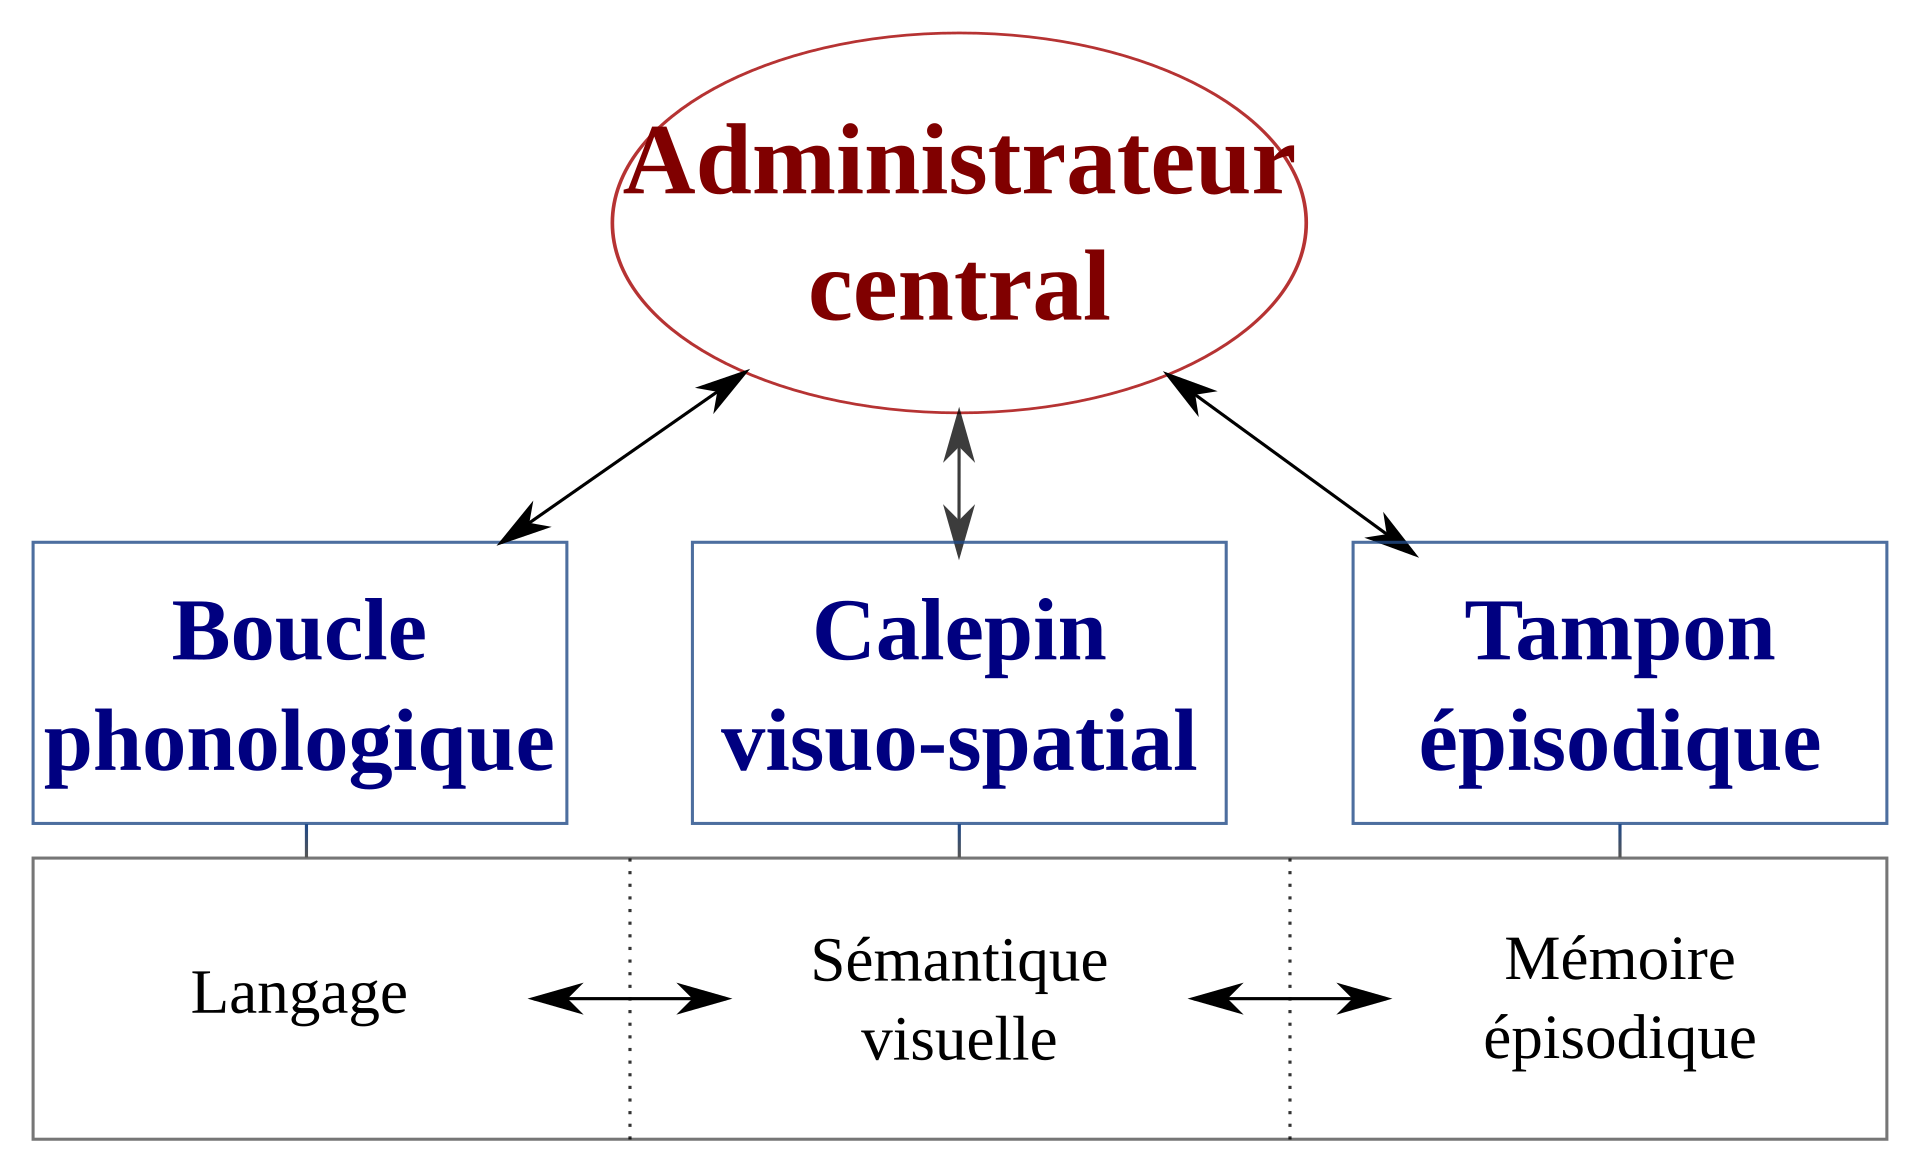
\includegraphics[width=0.7\textwidth]{images/modele_baddeley_hitch.png}
    \caption{Schéma du modèle de la mémoire de travail selon Baddeley et Hitch}
    \label{fig:baddeley}
\end{figure}

\newpage
Contrairement à la mémoire à court terme (MCT), \textbf{la mémoire à long terme (MLT)} stocke les informations de manière potentiellement illimitée et pour une durée prolongée. Elle permet d'accumuler des connaissances, des expériences et des souvenirs sur plusieurs années.

\textbf{Types de mémoire à long terme :}
\begin{itemize}
    \item \textbf{Mémoire déclarative (explicite) :} Elle concerne les souvenirs accessibles à la conscience et pouvant être exprimés verbalement.
    \begin{itemize}
        \item \textbf{Mémoire épisodique :} Stocke des souvenirs personnels, tels que des événements vécus (par exemple, un anniversaire d'enfance).
        \item \textbf{Mémoire sémantique :} Contient des connaissances générales sur le monde (par exemple, savoir que la Tour Eiffel se trouve à Paris).
    \end{itemize}
    \item \textbf{Mémoire non déclarative (implicite) :} Elle fonctionne sans implication consciente et se manifeste par des habiletés motrices ou des automatismes.
    \begin{itemize}
        \item \textbf{Mémoire procédurale :} Responsable de l'apprentissage des gestes et des compétences (par exemple, faire du vélo).
        \item \textbf{Conditionnements et habitudes :} Permet de réagir de manière automatique à certains stimuli (par exemple, saliver à l'odeur d'un plat préféré).
    \end{itemize}
\end{itemize}

\begin{figure}[h]
    \centering
    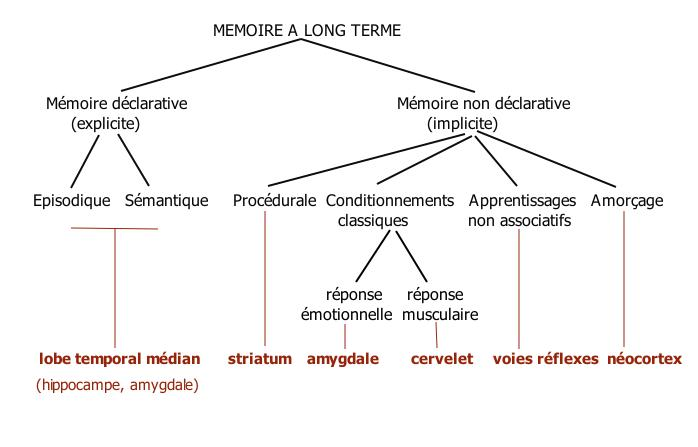
\includegraphics[width=0.7\textwidth]{images/types_memoire_long_terme.jpg}
    \caption{Représentation schématique des types de mémoire à long terme}
    \label{fig:mlt}
\end{figure}

\newpage
% 1.1.3
\subsection{Lien entre mémoire à court terme et mémoire à long terme}

La mémoire à court terme et la mémoire à long terme ne fonctionnent pas de manière indépendante, mais forment un système intégré. Le transfert d'informations entre ces deux systèmes est influencé par plusieurs facteurs, notamment :

\begin{itemize}
    \item \textbf{L'attention :} Une information qui capte fortement l'attention a plus de chances d'être stockée durablement.
    \item \textbf{La répétition :} La répétition espacée améliore la consolidation mnésique.
    \item \textbf{L'émotion :} Un événement émotionnellement marquant est plus susceptible d'être stocké dans la mémoire à long terme.
\end{itemize}

Des études ont montré que l'hippocampe, une structure cérébrale essentielle, joue un rôle clé dans le passage de la mémoire à court terme vers la mémoire à long terme.

https://www.francealzheimer.org/memoire-long-terme-court-terme/
https://www.mnpaf.fr/preserver-memoire/comment-fonctionne-notre-mémoire
https://www.humanite.fr/sciences/academie-des-sciences/lhippocampe-siege-de-la-memoire-et-gps-de-notre-cerveau
https://www.frcneurodon.org/comprendre-le-cerveau/a-la-decouverte-du-cerveau/la-memoire/





\section{Les troubles de la mémoire et leurs impacts}
Vieillissement cognitif et maladies neurodégénératives (Alzheimer, Parkinson)
Troubles de l'attention et de l'apprentissage (TDAH, dyslexie)
Surcharge cognitive et oubli informationnel
\section{Besoins et solutions existantes pour améliorer la mémorisation}
Méthodes traditionnelles (mnémoniques, répétition espacée)
Utilisation des technologies numériques actuelles
Limites des approches classiques
\chapter{L'intelligence artificielle au service de la mémorisation}
\section{Présentation des technologies d'IA utilisées pour l'assistance cognitive}
Traitement du langage naturel (NLP)
Apprentissage automatique et adaptatif
Reconnaissance vocale et synthèse de la parole
\section{Les assistants intelligents pour la mémoire}
Présentation des outils et applications existantes
Assistants vocaux (Siri, Alexa, Google Assistant)
Systèmes de rappel intelligents (Google Keep, Todoist avec IA)
Applications de mémorisation (Anki, Memrise, Duolingo)
Fonctionnement et personnalisation des réponses en fonction des utilisateurs
\section{Avantages et limites de l'IA dans l'amélioration de la mémoire}
Amélioration de la rétention et de l'accessibilité de l'information
Adaptabilité et personnalisation
Risques et limites : dépendance technologique, confidentialité, biais algorithmiques
\chapter{Applications concrètes et enjeux éthiques}
\section{L'IA dans l'éducation et l'apprentissage adaptatif}
Plateformes intelligentes pour l'éducation (Khan Academy, Coursera avec IA)
Personnalisation de l'apprentissage en fonction des performances de l'utilisateur
Suivi et analyse des progrès
\section{L'IA pour les personnes atteintes de troubles cognitifs}
Outils pour les seniors et les malades d'Alzheimer
Aide aux personnes atteintes de TDAH ou de dyslexie
Interfaces cerveau-ordinateur pour compenser les déficiences mnésiques
\section{Enjeux éthiques et défis techniques}
Confidentialité des données et respect de la vie privée
Fiabilité et contrôle des algorithmes
Accessibilité et inclusion : l'IA peut-elle être universellement efficace ?

% Conclusion
\chapter*{Conclusion}
\addcontentsline{toc}{chapter}{Conclusion}
hdsgc fkjhdsbf shgffskhg fkshgkjfsk\footnote{Ceci est une note de bas de page.}

Récapitulatif des apports de l'IA dans l'amélioration de la mémorisation
Perspectives d'évolution des technologies IA dans ce domaine
Limites et pistes d'amélioration
Réflexion sur l'impact futur des assistants intelligents dans la cognition humaine



% Postface (optionnel)
\chapter*{Postface}
\addcontentsline{toc}{chapter}{Postface}

% Bibliographie
\chapter*{Bibliographie}
\addcontentsline{toc}{chapter}{Bibliographie}

% Annexes (si nécessaire)
\chapter*{Annexes}
\addcontentsline{toc}{chapter}{Annexes}

\end{document}